%!TEX root=../document.tex
\section{Allgemein - Continous Integration}
Kontinuierliche Integration (Continuous Integration) ist eine Praxis in der Softwareentwicklung. Dabei werden isolierte Änderungen sofort geprüft und anschließend zur Gesamtcodebasis einer Software hinzugefügt. Ziel der kontinuierlichen Integration ist es, ein unmittelbares Feedback bieten zu können, so dass ein versehentlich integrierter Fehler so schnell wie möglich identifiziert und korrigiert wird. Tools für kontinuierliche Integration lassen sich dazu verwenden, Tests zu automatisieren und um eine fortlaufende Dokumentation zu erstellen.

Kontinuierliche Integration wurde in den letzten Jahren permanent weiterentwickelt. Ursprünglich war ein täglicher Build (täglicher Erstellungsprozess) Standard. Mittlerweile hat sich der Ansatz etabliert, regelmäßigere Builds zu erstellen - zum Beispiel so bald ein bestimmter Arbeitsschritt fertiggestellt ist.

Wird kontinuierliche Integration richtig angewandt, bietet der Ansatz verschiedene Vorteile, wie zum Beispiel ständige Feedbacks zum Status einer Software. Da sich mit kontinuierlicher Integration Mängel bereits in einem frühen Entwicklungsstadium erkennen lassen, fallen Softwarefehler kleiner sowie weniger komplex aus und lassen sich einfacher beseitigen.

\subsection{Continous Integration mit Jenkins}
Jenkins ist eine Software, welche das Prinzip Continous Integration ermöglicht.

Jenkins wird auf einem Server (localhost auch möglich) installiert, wo der Build Zentral stattfindet
\begin{figure}[!h]
\centering
\includegraphics[width=0.23\linewidth]{../../../../../../../../../../Shared/Jenkins/a02-tdd-bruch/Protokoll/Latex-files/images/jen}
\caption{Jenkins}
\label{fig:jen}
\end{figure}

\clearpage

\section{Ergebnisse}
\subsection{Installieren/Konfigurieren von Jenkins}
Jenkins ist für fast alle Plattformen erhältlich. Nach der Installation von Jenkins wird auf localhost unter 8080 ein Webserver gestartet, über welchen Jenkins konfiguriert werden kann.

Zu erst muss ein automatisch generiertes Passwort, welches sich in dem erstellten jenkins Logfile befindet, eingegeben werden. In meinem Fall befand sich das Logfile unter \texttt{/var/log/jenkins}

\subsubsection{Konfigurieren und Installieren der Plugins}
\paragraph{Manage Jenkins/ Github Support}\mbox{}
\vspace{0.16cm}

Unter \textit{Manage Jenkins > Configure System} unter dem Punkt \textbf{Git plugin} kann der Username sowie die email Addresse global gesetzt werden.
\begin{figure}[!h]
\centering
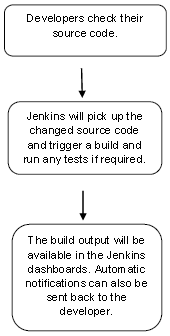
\includegraphics[width=1\linewidth]{../../../../../../../../../../Shared/Jenkins/a02-tdd-bruch/Protokoll/Latex-files/images/s1}
\caption{Username setzen / Git}
\label{fig:s1}
\end{figure}

\paragraph{Benötigte Plugins}\mbox{}
\vspace{0.16cm}

Um alle Anforderungen zu erfüllen müssen mindestens folgende Plugins installiert werden.
\begin{itemize}
	\item Violations
	\item GitHub Integration Plugin
	\item Cobertura Plugin
\end{itemize}

Um ein Plugin zu installieren, muss zu folgender Seite navigiert werden\\ \textit{Manage Jenkins > Manage Plugin > Available}\\
Nach der Installation eines Plugins sollte Jenkins neugestartet werden.

\subsection{Erstellen eines neuen Jobs}
Nach der Konfiguration kann ein neuer Job/Item erstellt werden.
Folgende Schritte sind hierbei zu beachten.
\begin{itemize}
	\item \textbf{Projekt Typ auswählen}\\
	Eingabe des Projektnamen, sowie Auswahl des Typs
	\begin{figure}[!h]
		\centering
		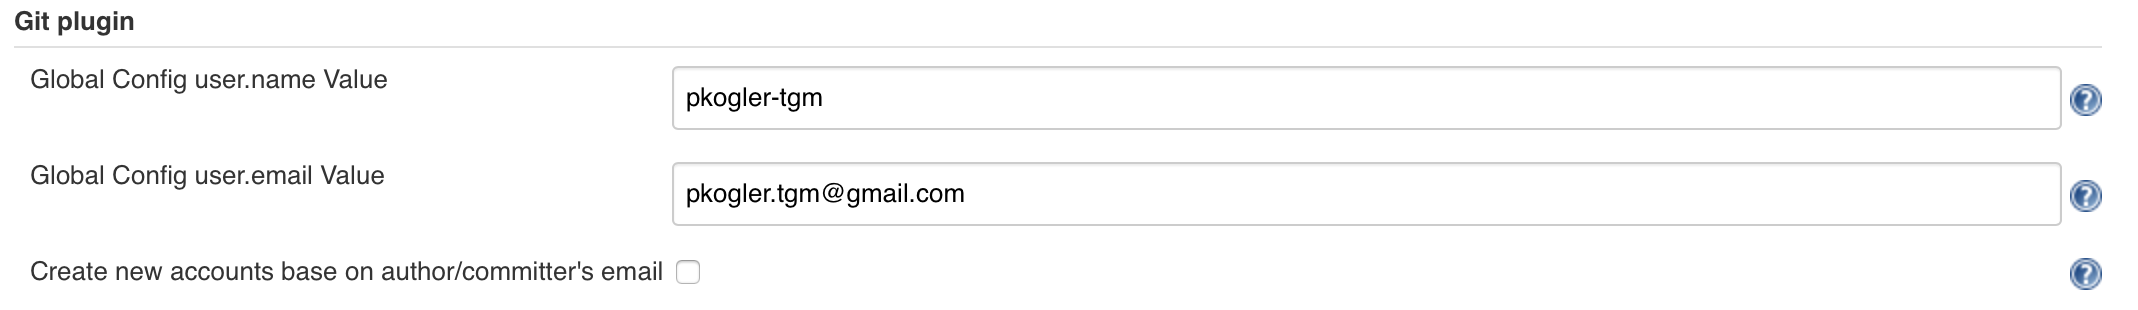
\includegraphics[width=0.9\linewidth]{../../../../../../../../../../Shared/Jenkins/a02-tdd-bruch/Protokoll/Latex-files/images/s2}
		\label{fig:s2}
	\end{figure}
	
	\item \textbf{Source Code Management}\\
	Angabe des Projekt Pfaded hier GitHub Integration
	\begin{figure}[!h]
		\centering
		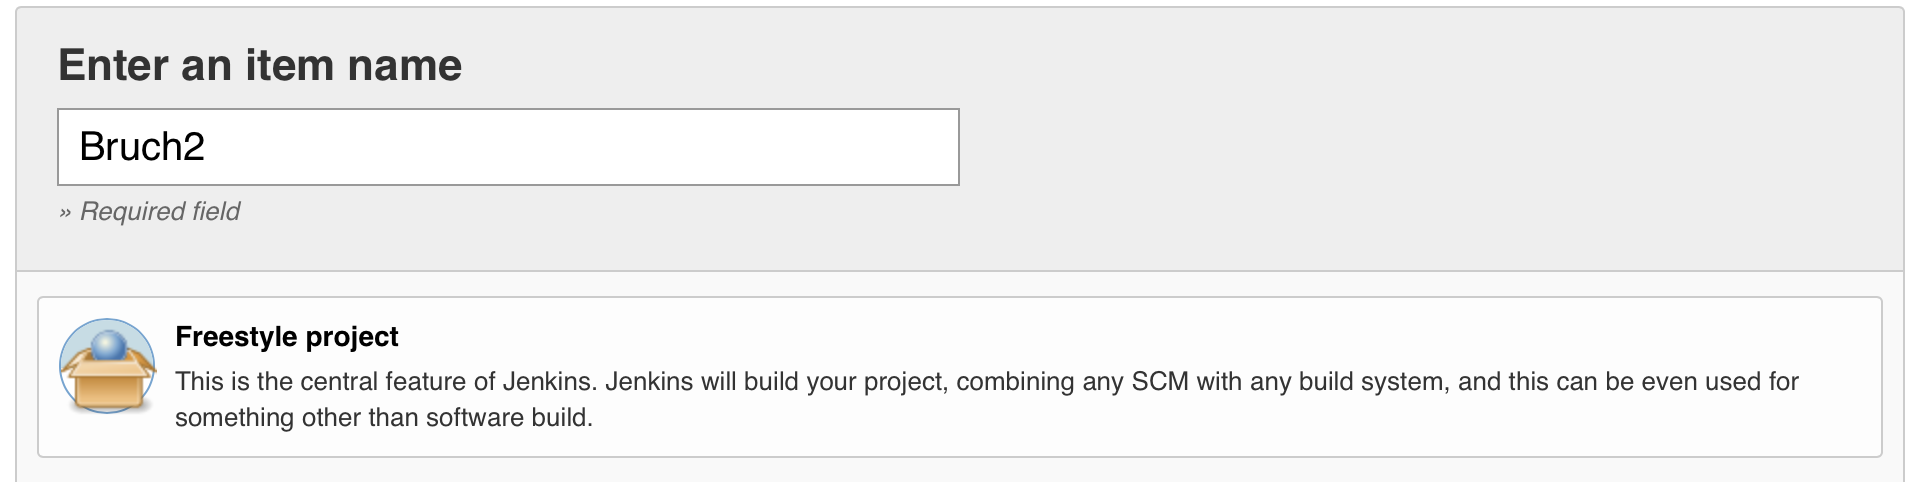
\includegraphics[width=0.9\linewidth]{../../../../../../../../../../Shared/Jenkins/a02-tdd-bruch/Protokoll/Latex-files/images/s3}
		\label{fig:s3}
	\end{figure}
	In meinem Fall wird ein lokales Repository genutzt. Damit das erfolgreich eingerichtet werden kann und Jenkins somit Zugriff auf dieses Repo hat, kann ein neuer ssh Key generiert werden und auf Github regestriert werden.
	\begin{figure}[!h]
		\centering
		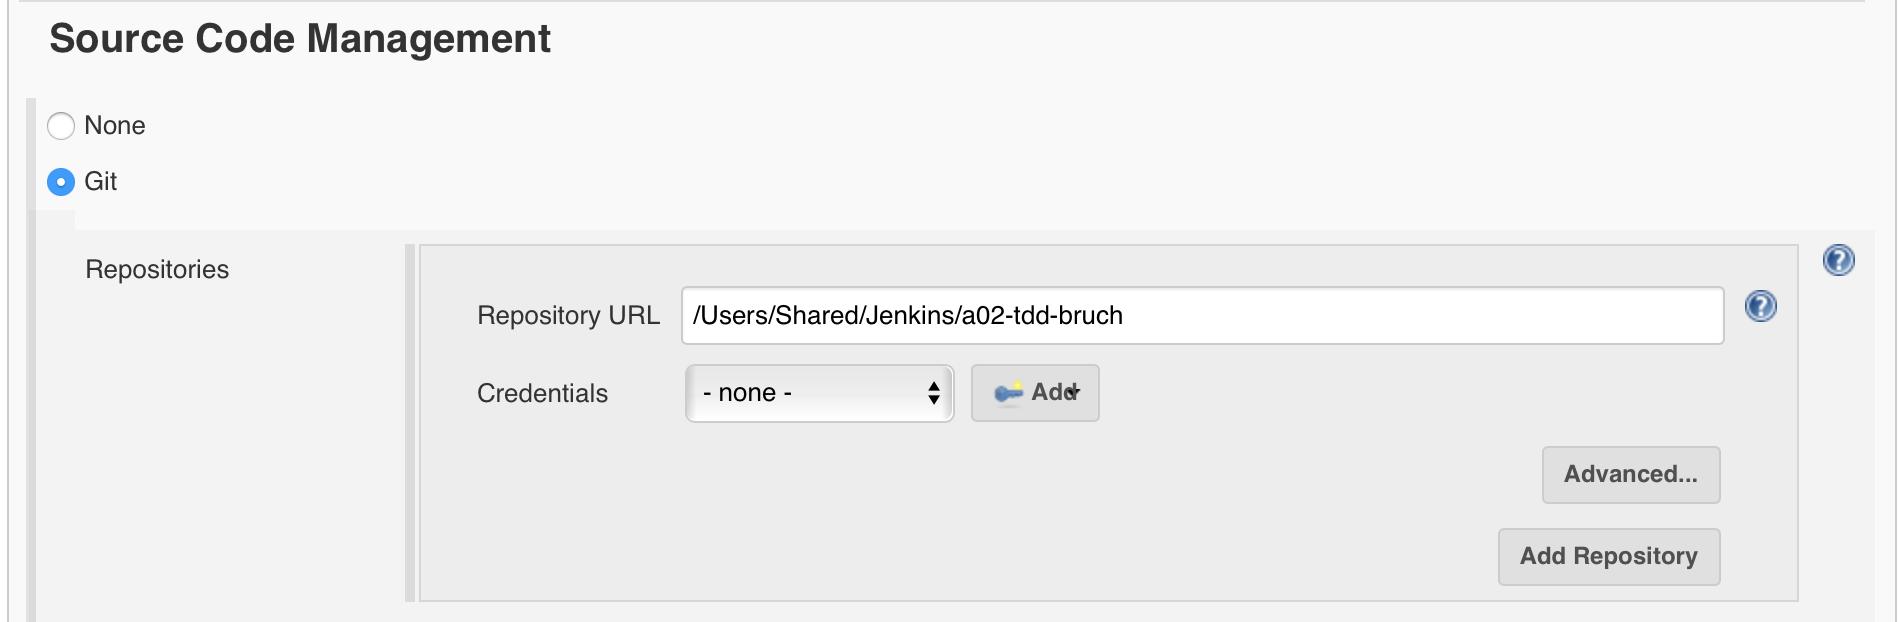
\includegraphics[width=0.9\linewidth]{../../../../../../../../../../Shared/Jenkins/a02-tdd-bruch/Protokoll/Latex-files/images/s4}
		\label{fig:s4}
	\end{figure}
	
	\clearpage
	
	\item \textbf{Build Triggers}\\
	Anschließend können ein oder mehrere Build Trigger gesetzt werden. Also nach welcher Aktion/Aktionen ein Build gestartet werde soll. In unserem Fall wurde ein SCM Trigger gesetzt, welcher alle 5 min einen automatischen Build startet.
	\begin{figure}[!h]
		\centering
		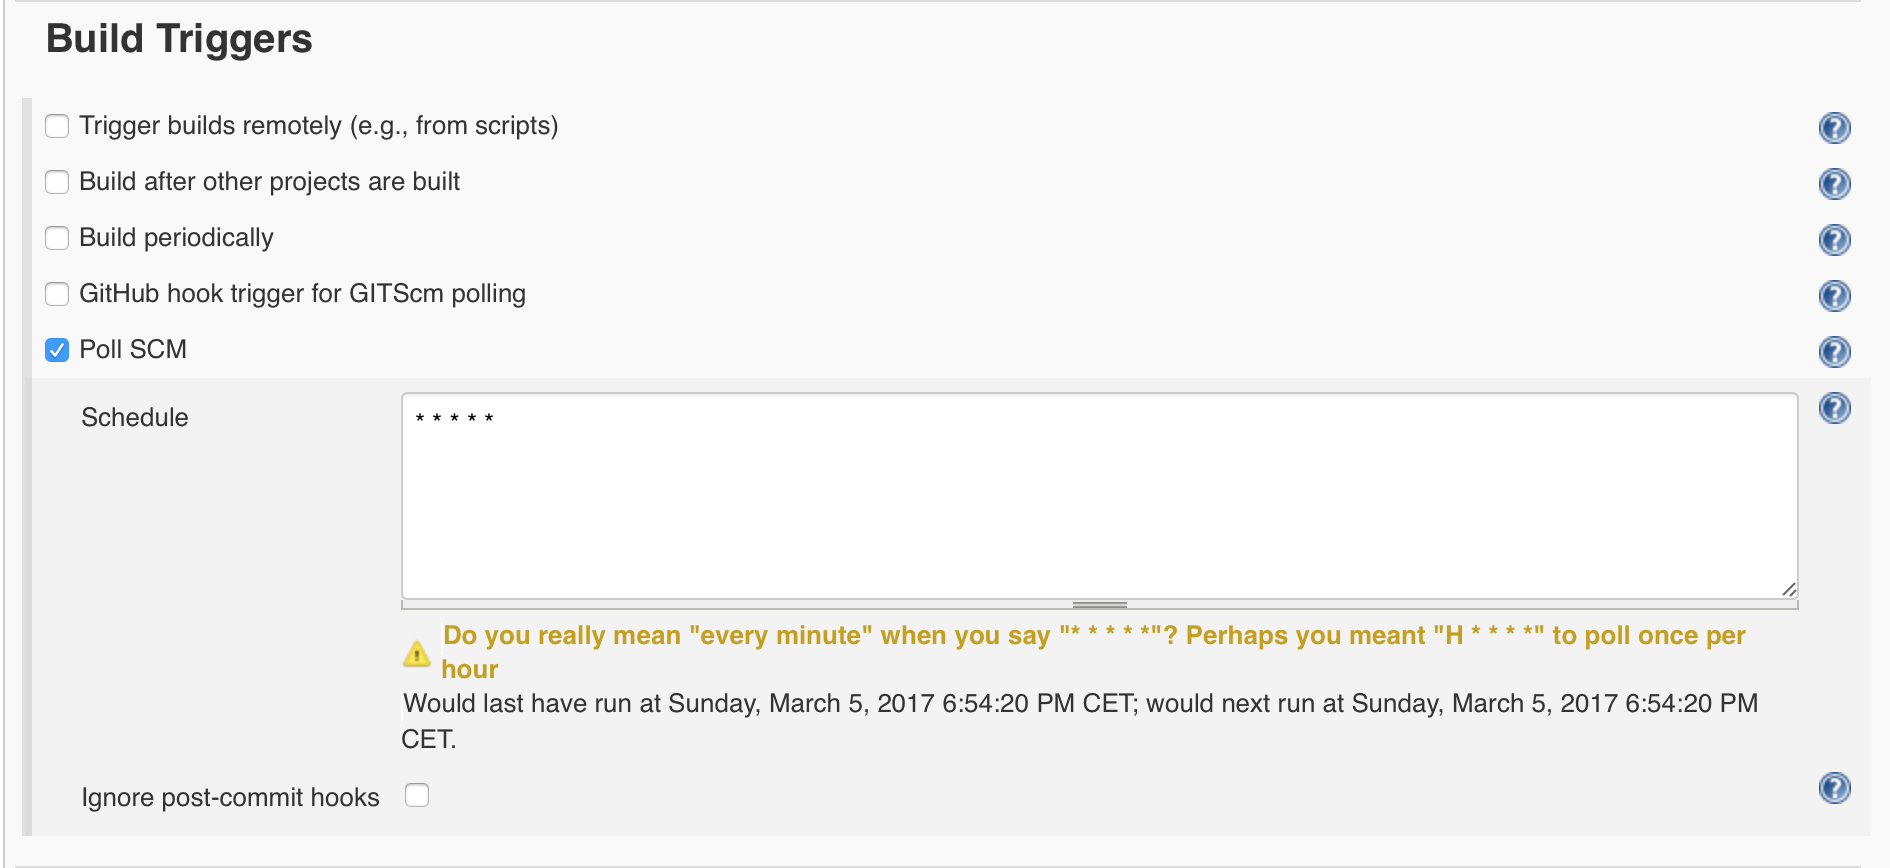
\includegraphics[width=0.9\linewidth]{../../../../../../../../../../Shared/Jenkins/a02-tdd-bruch/Protokoll/Latex-files/images/s5}
		\label{fig:s5}
	\end{figure}
	
	\item \textbf{Build Configuration}\\
	Der eigentliche Build kann nun in als \textit{Execute Shell} beschrieben und definiert werden. Alle auszuführenden Kommandos werden in dem angegeben Verzeichnis angegeben.
	\begin{figure}[!h]
		\centering
		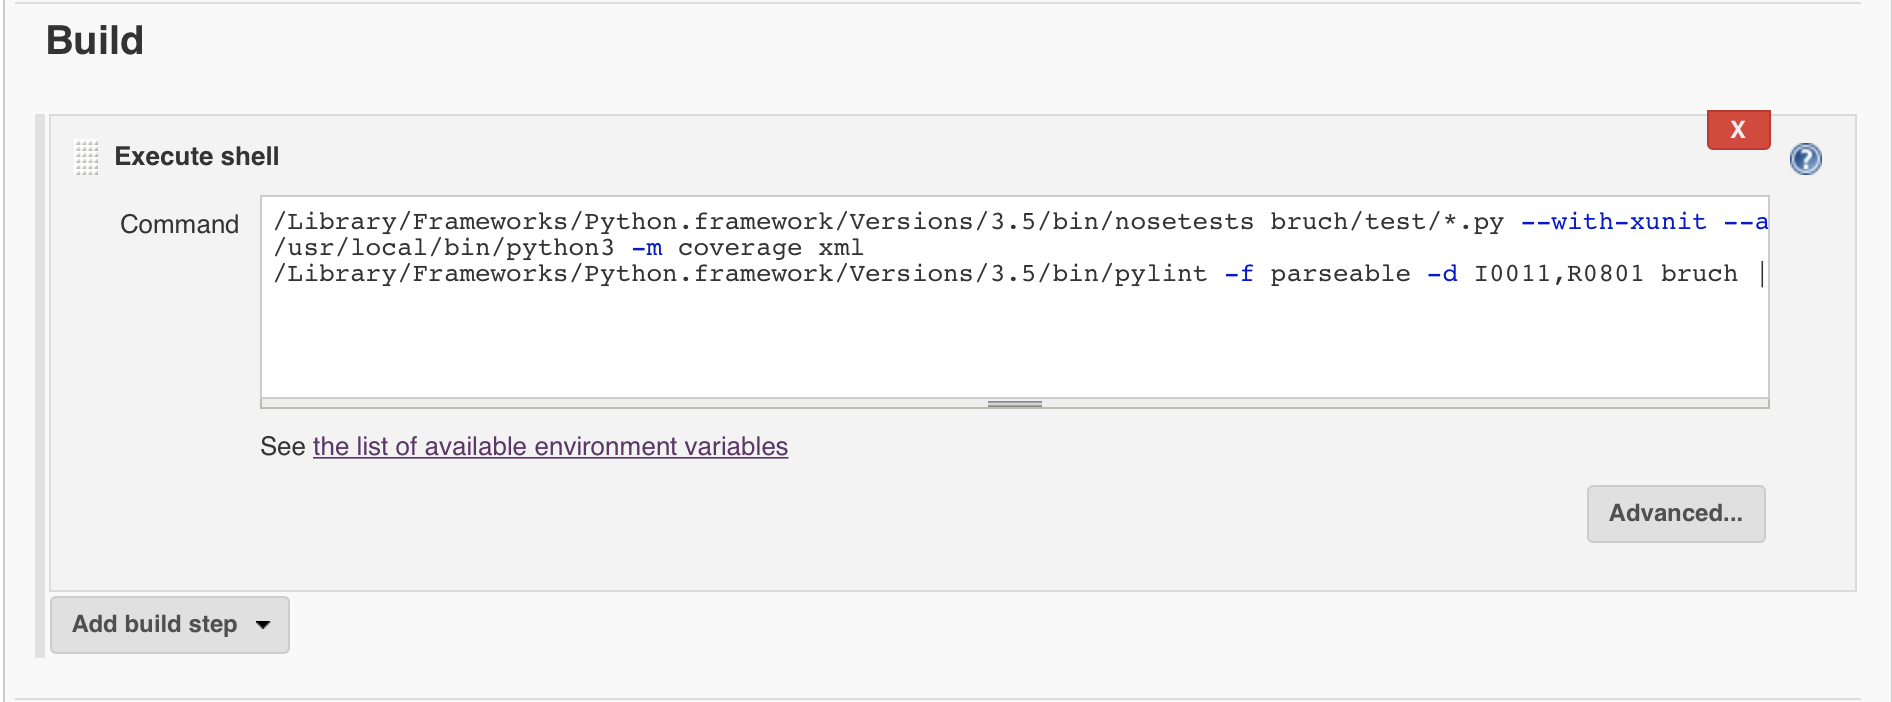
\includegraphics[width=0.9\linewidth]{../../../../../../../../../../Shared/Jenkins/a02-tdd-bruch/Protokoll/Latex-files/images/s6}
		\label{fig:s6}
	\end{figure}\\
	\textbf{.../nosetests} \hspace{0.7cm} bruch/test/*py erstellt ein xml file welches später interpretiert werden kann\\
	\textbf{./python cov} \hspace{0.5cm} erstellt einen coverage report als xml\\
	\textbf{.pylint parse} \hspace{0.5cm} analysiert das modul bruch\\
	
	\clearpage
	
	\item \textbf{Post Build Configuration}\\
	Anschließend können diese Build Ergebnisse als Post Build Script ausgewertet werden. Also nach einem erfolgreichem Build können bestimmte Befehle ausgeführt werden.
	
	Auswerten der erstellten Reports. Alle ausgewerteten Berichte sind im XML Format und können so ausgewertet werden.
	\begin{figure}[!h]
		\centering
		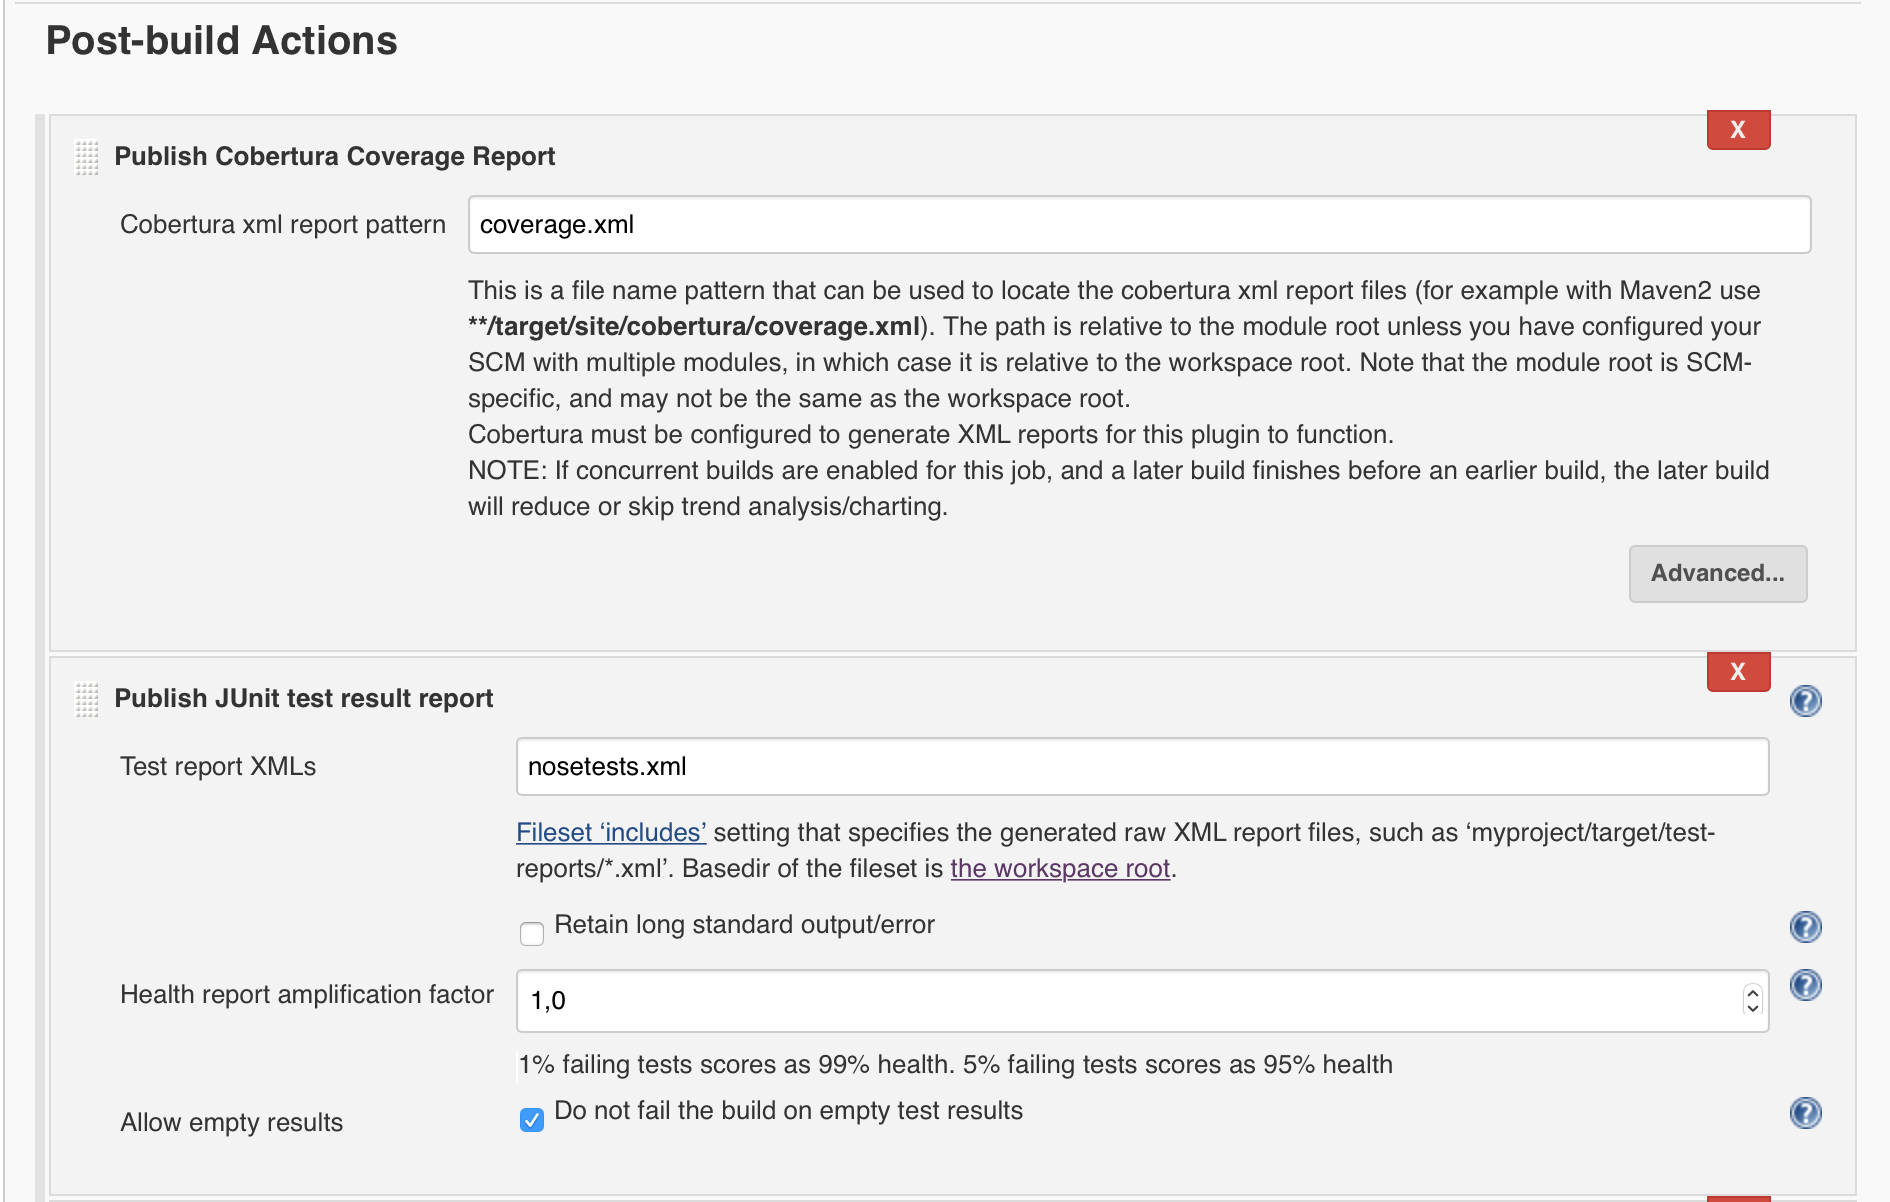
\includegraphics[width=0.9\linewidth]{../../../../../../../../../../Shared/Jenkins/a02-tdd-bruch/Protokoll/Latex-files/images/s7}
		\label{fig:s7}
	\end{figure}
	Ebenfalls soll das Ergebnis von pylint dargestellt werden. Dies kann mithilfe des generierten \textit{pylint.out} umgesetzt werden.
	\begin{figure}[!h]
		\centering
		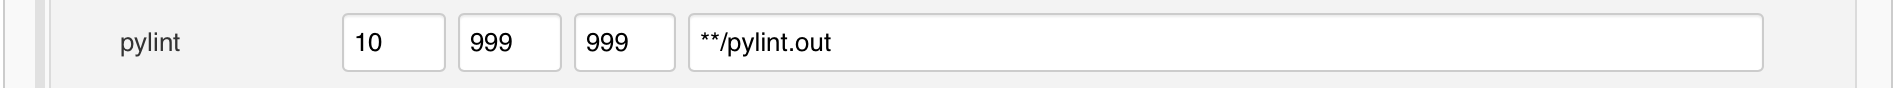
\includegraphics[width=0.9\linewidth]{../../../../../../../../../../Shared/Jenkins/a02-tdd-bruch/Protokoll/Latex-files/images/s8}
		\label{fig:s8}
	\end{figure}
\end{itemize}

\clearpage
\subsection{Durchführen eines Builds}
EIn Build kann auch manuell durchgeführt werden. Um diesen einzuleiten muss wie folgt vorgegangen werden.
\begin{figure}[!h]
	\centering
	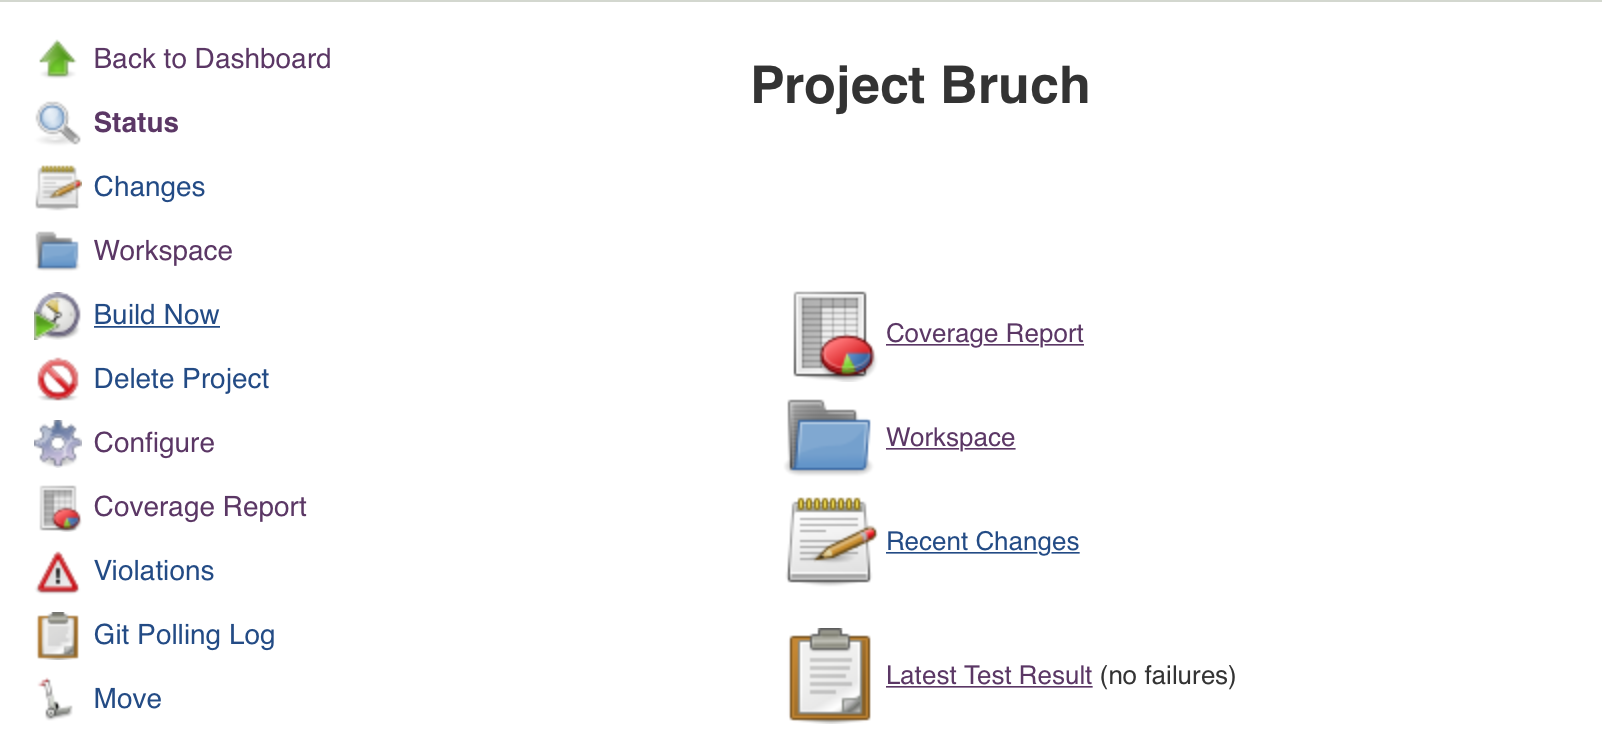
\includegraphics[width=0.9\linewidth]{../../../../../../../../../../Shared/Jenkins/a02-tdd-bruch/Protokoll/Latex-files/images/s9}
	\label{fig:s9}
\end{figure}
\clearpage
\subsection{Build Report und Auswertung}
Nach jedem erfolgreichem Build (gekennzeichnet mit einem Blauen Punkt) wird das dazugehörige Post Build Script ausgeführt. In unserem Fall werden sowohl die Testberichte als auch der Coverage Bericht ausgewertet. Ebenfalls wird mittels pylint eine kurze Code Analyse durchgeführt.

\subsubsection{Übersicht des Reports}
Aufgeteilt in Änderungen, Git Report, Coverage Report und Test Results
\begin{figure}[!h]
	\centering
	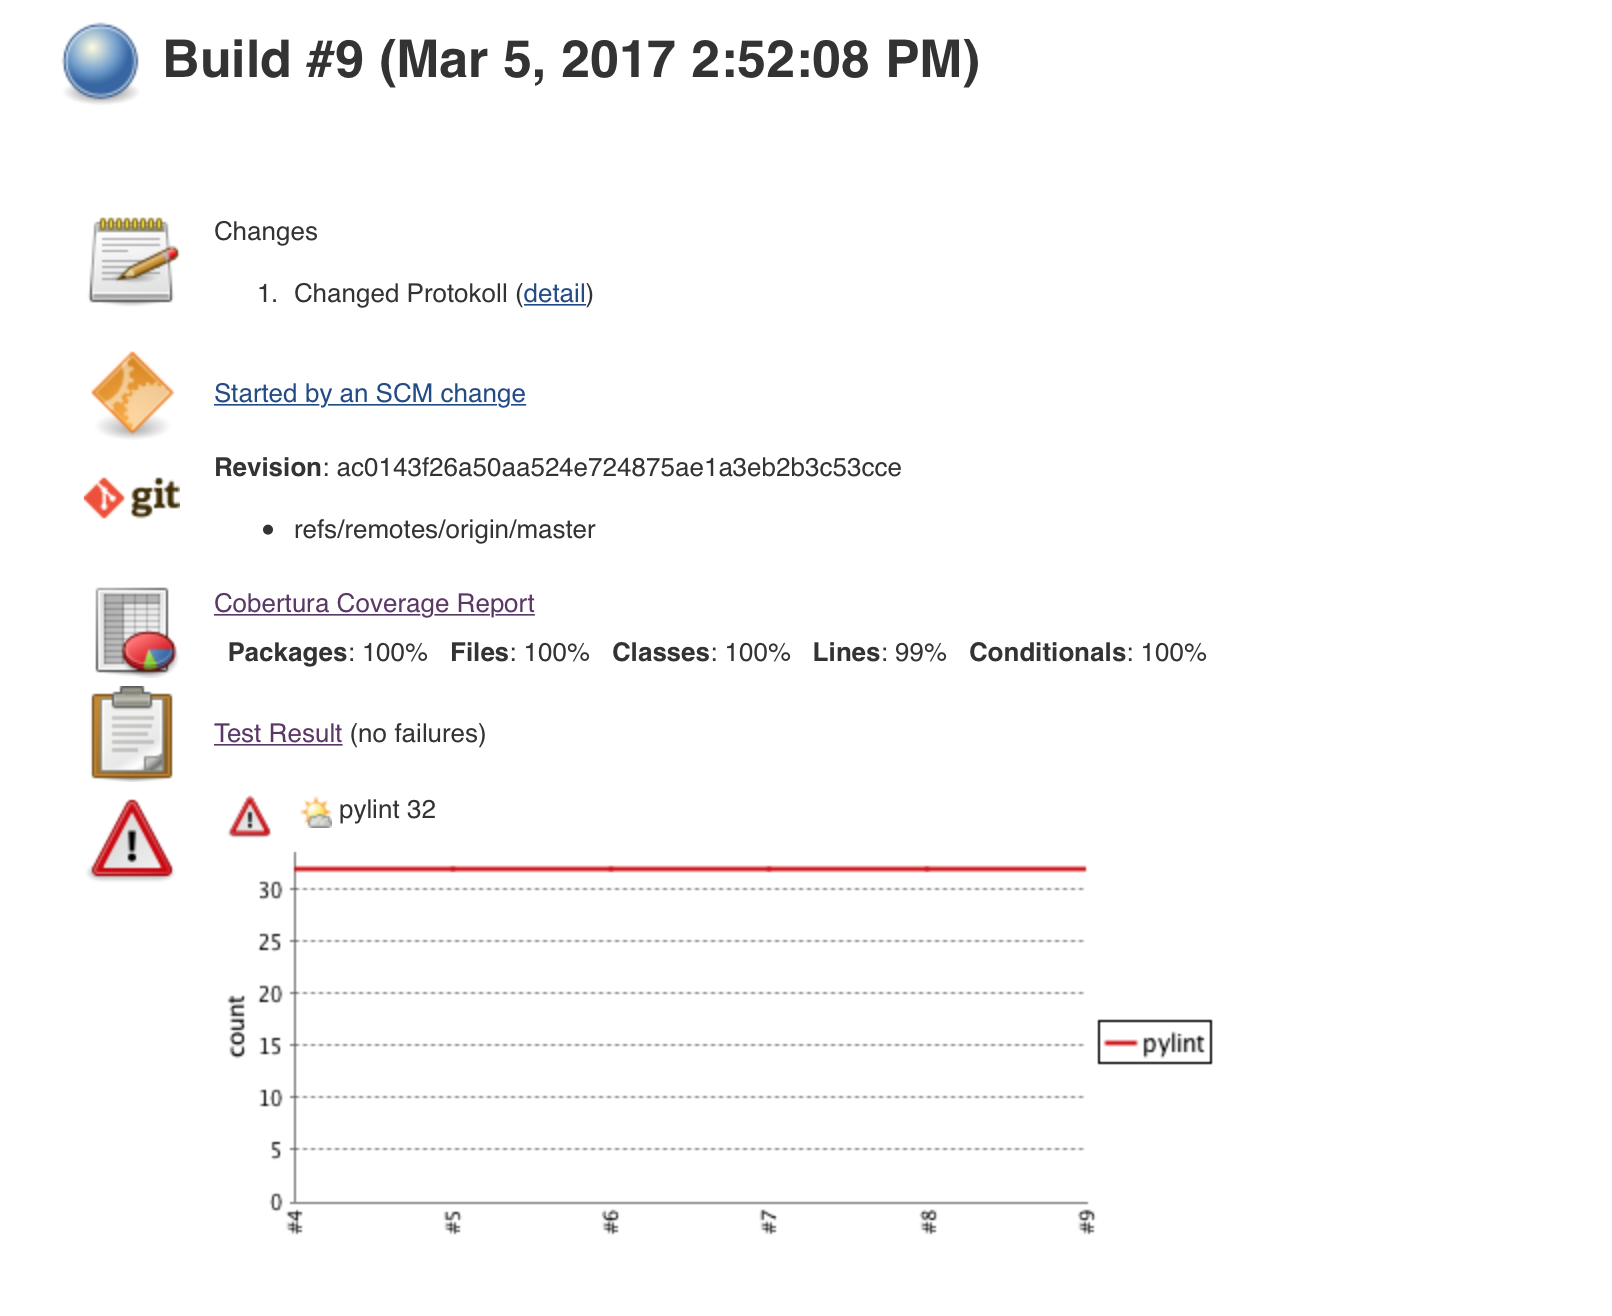
\includegraphics[width=0.9\linewidth]{../../../../../../../../../../Shared/Jenkins/a02-tdd-bruch/Protokoll/Latex-files/images/s10}
	\label{fig:s10}
\end{figure}

\subsubsection{Coverage Report}
\begin{figure}[!h]
	\centering
	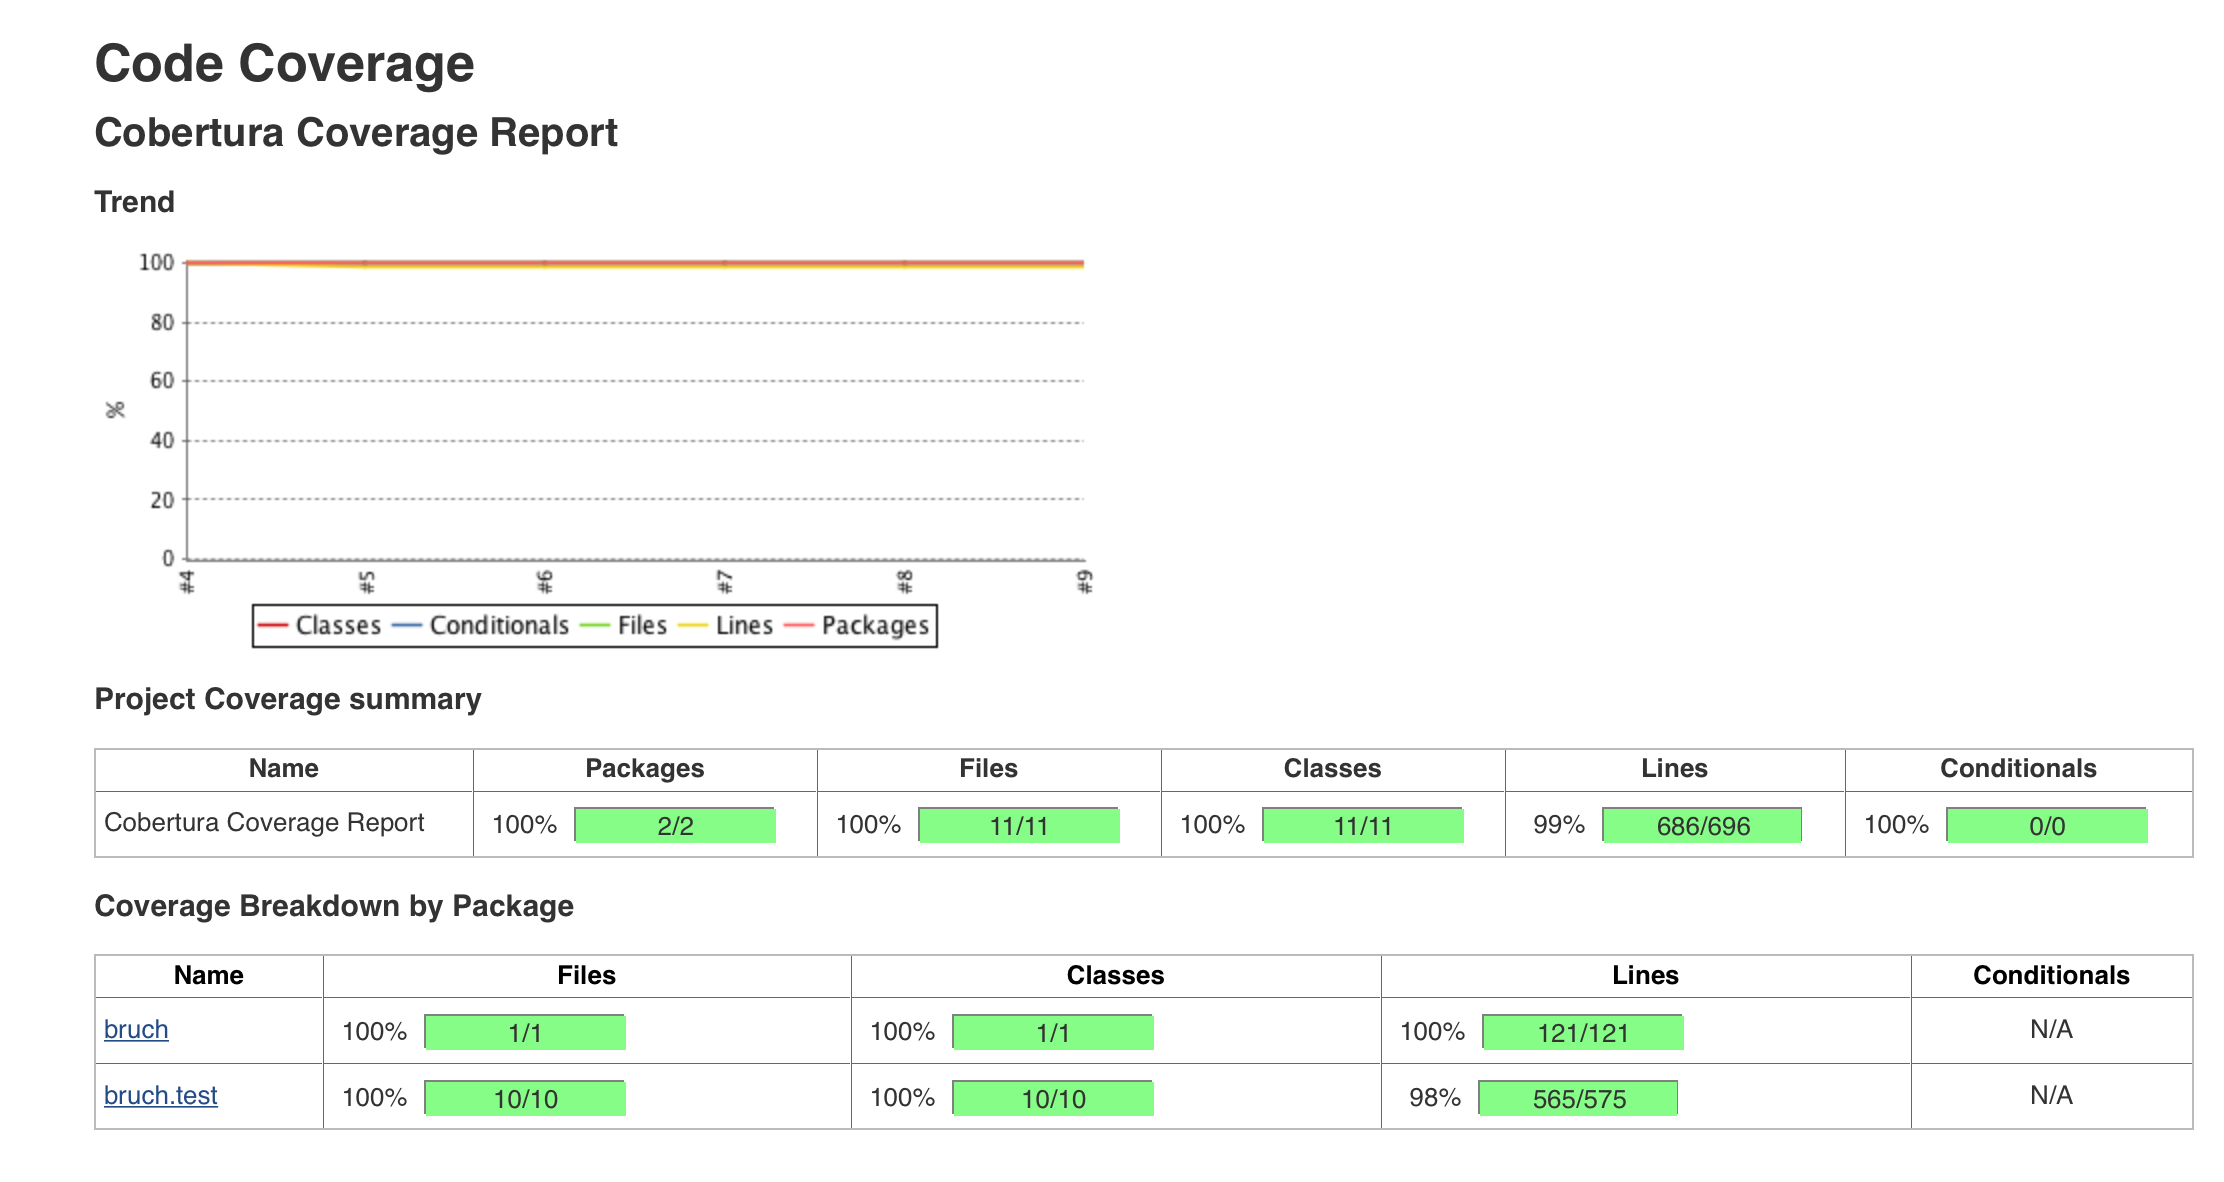
\includegraphics[width=0.9\linewidth]{../../../../../../../../../../Shared/Jenkins/a02-tdd-bruch/Protokoll/Latex-files/images/s11}
	\label{fig:s11}
\end{figure}

\subsubsection{Test Reports}
Alle durchgeführten Tests werden ebenfalls dargestellt.\\
Die Navigation erfolgt ähnlich wie bei normalen (html) exportierten Unit Tests
\begin{figure}[!h]
	\centering
	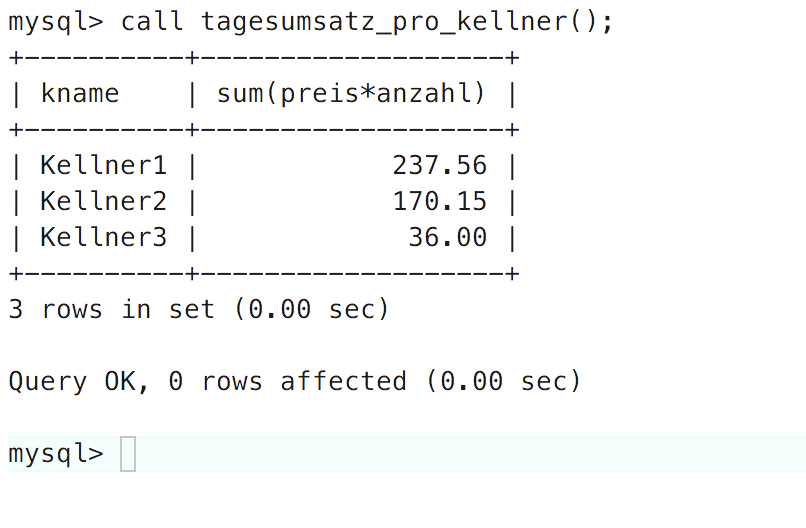
\includegraphics[width=0.9\linewidth]{../../../../../../../../../../Shared/Jenkins/a02-tdd-bruch/Protokoll/Latex-files/images/s12}
	\label{fig:s12}
\end{figure}

\subsubsection{Pylint Reports}
Die Violation Reports können mit pylint durchgeführt werden. Hierbei werden vor allem Die Richtlinien nach dem Styleguide von Python \textbf{PEP 8} beachtet.
\begin{figure}[!h]
	\centering
	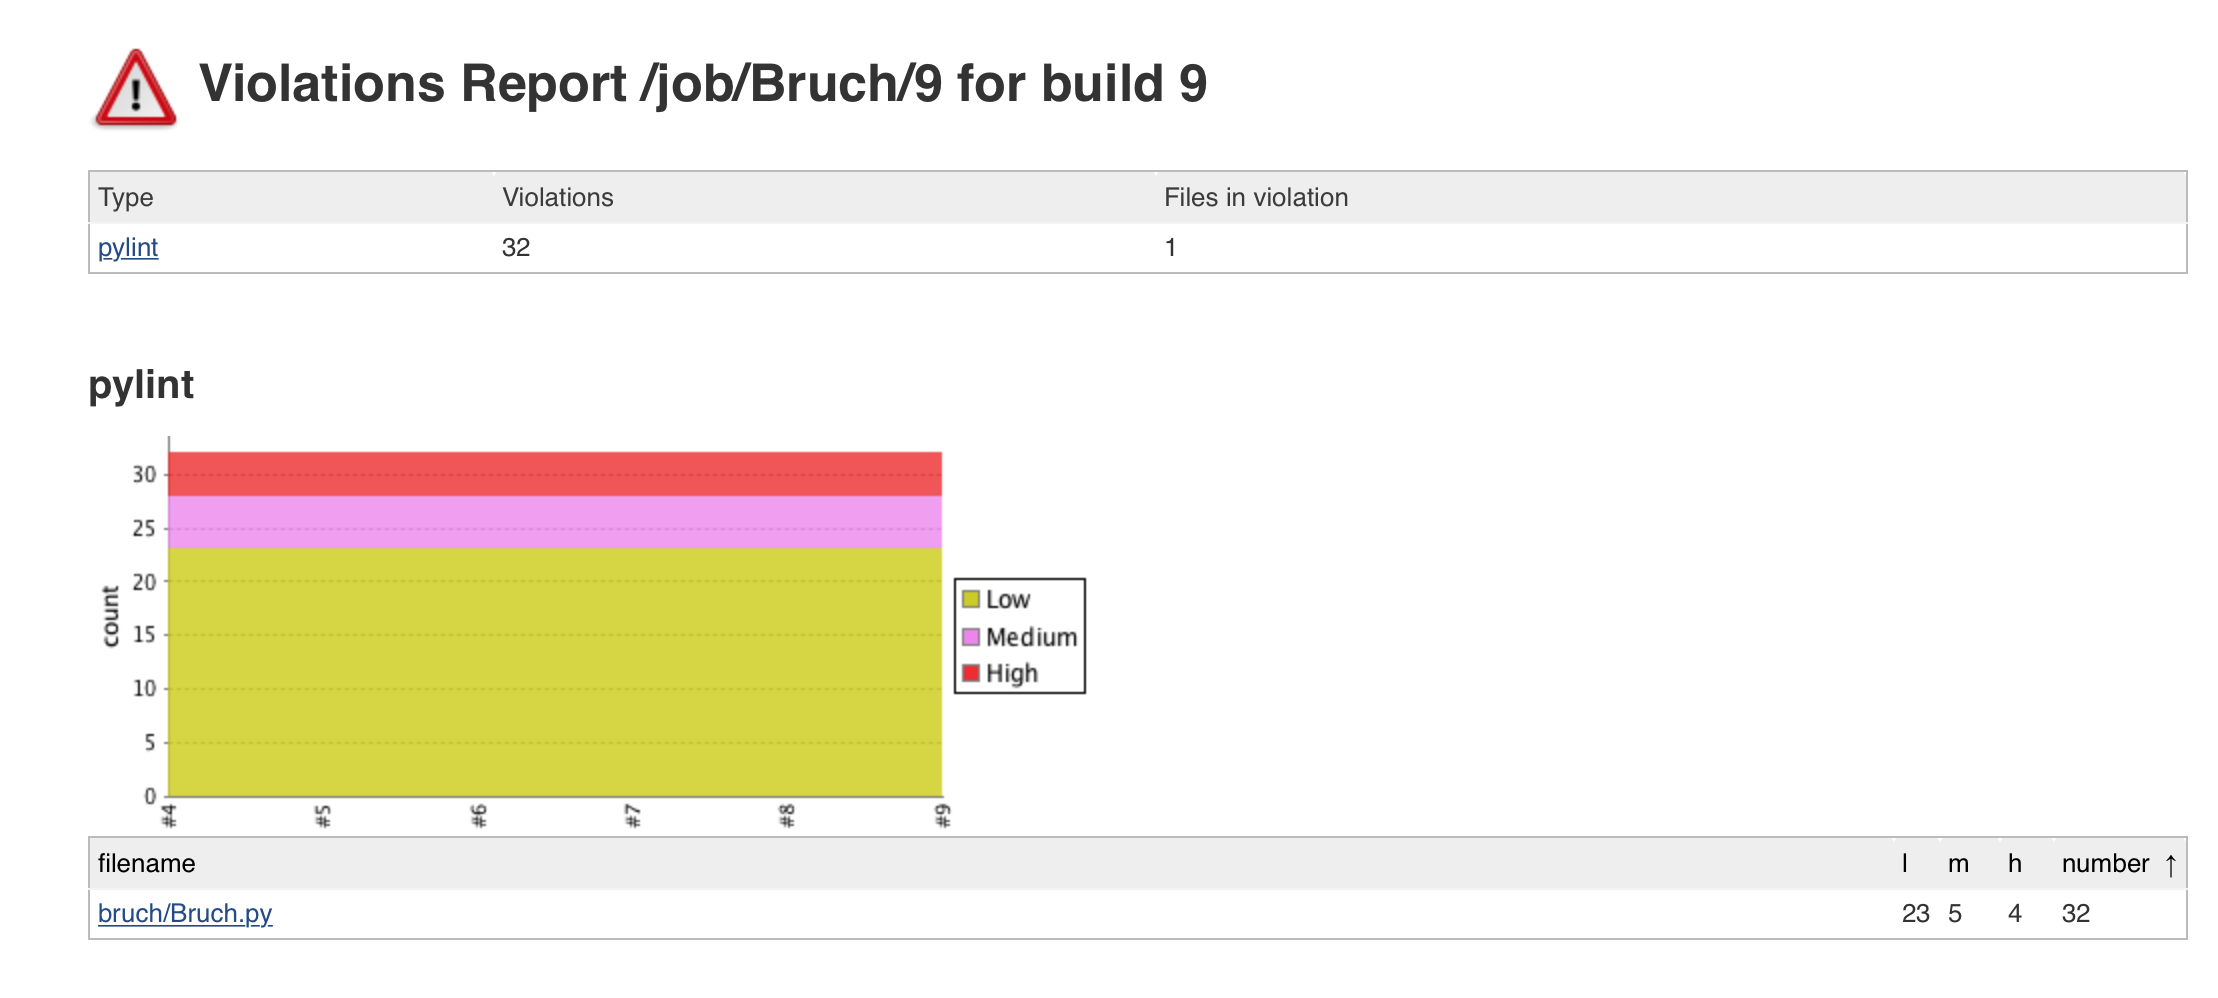
\includegraphics[width=0.9\linewidth]{../../../../../../../../../../Shared/Jenkins/a02-tdd-bruch/Protokoll/Latex-files/images/s13}
	\label{fig:s13}
\end{figure}

\subsection{Aufgetretene Probleme}
Das Installieren von Jenkins war sehr einfach und aufgrund der gut ausgeführten Dokumentation sowie der relativ großen Community unkompliziert umzusetzen.

Auch das Erstellen des Items war nicht weiter schwierig. Jedoch sind Probleme beim Erstellen der Build Konfiguration aufgetreten. Da alle Befehle direkt von dem erstellten jenkins User durchgeführt werden, muss darauf geachtet werden, dass dieser die Berechtigungen für alle notwendigen Befehle hat. 

Beispielsweise wurden exportierte Aliases nicht für den User übernommen.
Als Lösung wurde der Pfad absolut angegeben und auf diese benötigten Scripts dementsprechende Berechtigungen vergeben.

Das Installieren von nose und pylint ist ebenfalls sehr einfach verlaufen. Jedoch wurde unter OSX nosetest nicht in die PATH Variable aufgenommen. Nach Lokation des bin Verzeichnisses von Python, war die Verlinkung jedoch kein Problem mehr.
\clearpage 
\subsection{GUI - Testing mit Jenkins}
Nach einer ausführlichen Recherche über das oben genannte Thema bin ich auf folgende Ergebnisse gekommen.

GUI - Testing an sich ist mit Jenkins selbstverständlich möglich, jedoch sind die Möglichkeiten sehr eingeschränkt. Beispielsweise kann unabhängig von OS und zu testender Programmiersprache (sofern solche Tools für die Programmiersprache vorhanden sind), ein Script ausgeführt werden welches das Programm startet und beispielsweise Deskription und Initialisierungswerte der GUI abfragt und dementsprechend in einem XML File ablegt. Dieses kann anschließend von Jenkins ausgewertet werden. 

\subsubsection{QF-Test Plugin \cite{qfs}}
Diese Plugin für Jenkins ermöglicht das Testen von GUI - Applikationen.
Hierbei können jedoch nur Java Applikationen getestet werden. (JavaFX, Swing) und Java EE Applikationen.

\subsubsection{Python GUI Testing mit Selenium \cite{py}}
Um eine Python Applikation kann beispielsweise Selenium verwendet werden. Ein ausführliches Tutorial wie so ein Test Job durchgeführt werde kann wird in diesem Blog Post beschrieben. \cite{py}

\section{Zeitaufwand}
\renewcommand{\arraystretch}{1.5}
\begin{table}[!h]
	\center
	\begin{tabular}{ |l|l|l|l| }
		\hline
		\textbf{Fertigstellung} & \textbf{Beschreibung} & \textbf{Geschätzte Zeit} & \textbf{Benötigte Zeit}\\ \hline \hline
		05.03..2017 & Installation von Jenkins & 50 min & 30 min\\ \hline
		05.03..2017 & Konfiguration von Jenkins & 50 min & 40 min\\ \hline
		05.03..2017 & Erstellen eines Jenkins Jobs & 130 min & 100 min\\ \hline
		05.03..2017  & Konfiguration des Builds& 40 min & 50 min\\ \hline
		05.03..2017  & Erweiterte Kompetenzen& 40 min & 50 min\\ \hline
		05.03..2017  & Protokoll & 100 min & 100 min\\ \hline \hline
		& \textbf{Insgesamt} & \textbf{290 min} & \textbf{310 min} \\ \hline
	\end{tabular}
	\caption{Zeitschätzung}
	\label{methoden}
\end{table}


\clearpage